\documentclass{article}
\usepackage[left=0.75in,top=0.65in,right=0.75in,bottom=0.55in]{geometry}

\usepackage{Sweave}
\begin{document}
\Sconcordance{concordance:report.tex:report.Rnw:%
1 5 1 49 0 1 6 11 1 1 5 2 1 1 18 6 1 7 0 7 1 7 0 6 1 7 0 6 1 7 0 6 %
1 7 0 6 1 7 0 6 1 7 0 2 1 1 11 4 1 11 0 3 1 1 18 6 1 7 0 7 1 7 0 6 %
1 7 0 6 1 7 0 6 1 7 0 6 1 7 0 6 1 7 0 2 1 1 11 4 1 11 0 3 1}

\title{Calculation of processing and overprocessing}
\date{}
\maketitle

\section{For Bondora log}
\begin{Schunk}
\begin{Sinput}
> result = read.csv("output_bondora_1.csv",header = TRUE)
\end{Sinput}
\end{Schunk}

Average number of checks that one would do if they follow \textbf{our ordering}:

\begin{Schunk}
\begin{Sinput}
> mean(result$nr_checks_our_suggestion)
\end{Sinput}
\begin{Soutput}
[1] 2.865327
\end{Soutput}
\end{Schunk}

Average number of checks that one would do if they apply \textbf{Wil's method} (constant reject probabilities):

\begin{Schunk}
\begin{Sinput}
> mean(result$nr_checks_wil)
\end{Sinput}
\begin{Soutput}
[1] 2.843984
\end{Soutput}
\end{Schunk}

Average number of checks that one would do if for every case they do checks in \textbf{random order}

\begin{Schunk}
\begin{Sinput}
> mean(result$nr_checks_random)
\end{Sinput}
\begin{Soutput}
[1] 2.796306
\end{Soutput}
\end{Schunk}

Average \textbf{overprocessing} - our method

\begin{Schunk}
\begin{Sinput}
> mean(result$nr_checks_our_suggestion - result$minimum_check_number)
\end{Sinput}
\begin{Soutput}
[1] 0.02446331
\end{Soutput}
\end{Schunk}

Average \textbf{overprocessing} - Wil method

\begin{Schunk}
\begin{Sinput}
> mean(result$nr_checks_wil - result$minimum_check_number)
\end{Sinput}
\begin{Soutput}
[1] 0.00312032
\end{Soutput}
\end{Schunk}

Average \textbf{overprocessing} - random ordering

\begin{Schunk}
\begin{Sinput}
> mean(result$nr_checks_random - result$minimum_check_number)
\end{Sinput}
\begin{Soutput}
[1] -0.04455816
\end{Soutput}
\end{Schunk}

\paragraph{Distribution of overprocessing}

\begin{Schunk}
\begin{Sinput}
> result$our = result$nr_checks_our_suggestion - result$minimum_check_number
> result$wil = result$nr_checks_wil - result$minimum_check_number
> result$rand = result$nr_checks_random - result$minimum_check_number
> tt = as.data.frame(cbind(table(result$our), table(result$wil), table(result$rand)))
> colnames(tt)=c("our","wil","rand")
> tt$overprocessing = rownames(tt)
> tt.m = melt(tt, id.vars='overprocessing')
> ggplot(tt.m, aes(overprocessing, value))+  geom_bar(aes(fill = variable), position = "dodge", stat="identity") + theme_grey(base_size = 18) + ylab("Nr of cases")
\end{Sinput}
\end{Schunk}
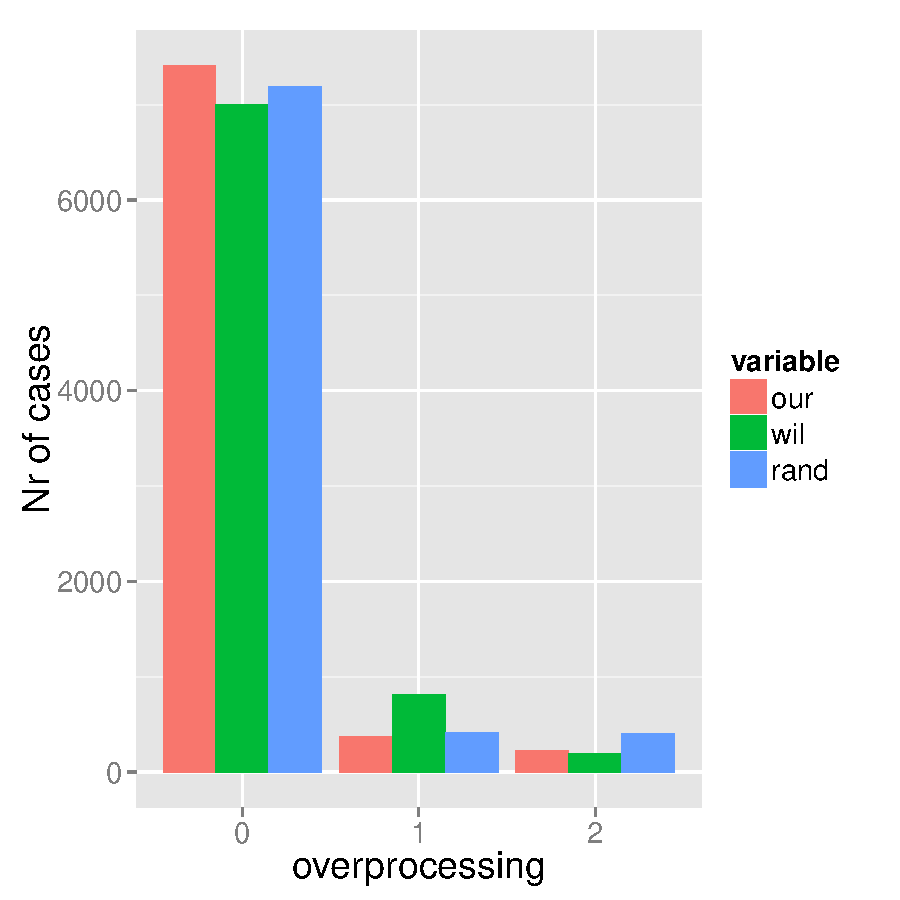
\includegraphics{report-009}


\section{For Environmental permit log}
\begin{Schunk}
\begin{Sinput}
> result = read.csv("output_envpermit_1.csv",header = TRUE,sep=",")